% Created 2020-11-12 四 20:08
% Intended LaTeX compiler: xelatex
\documentclass[11pt]{article}
\usepackage{graphicx}
\usepackage{grffile}
\usepackage{longtable}
\usepackage{wrapfig}
\usepackage{rotating}
\usepackage[normalem]{ulem}
\usepackage{amsmath}
\usepackage{textcomp}
\usepackage{amssymb}
\usepackage{capt-of}
\usepackage{hyperref}
\usepackage{ctex}
\author{Wang Jian}
\date{\today}
\title{BLINK: FAST AND GENERIC COLLECTIVES FOR DISTRIBUTED ML(MLSys 2020)}
\hypersetup{
 pdfauthor={Wang Jian},
 pdftitle={BLINK: FAST AND GENERIC COLLECTIVES FOR DISTRIBUTED ML(MLSys 2020)},
 pdfkeywords={},
 pdfsubject={},
 pdfcreator={Emacs 27.1 (Org mode 9.4)}, 
 pdflang={English}}
\begin{document}

\maketitle
\tableofcontents

\begin{abstract}
跨GPU的模型参数同步为大规模数据并行训练引入了高开销。面对不断增加的硬件异构性,现有的参数同步协议无法有效地利用可用的网络资源。我们提出Blink(a collective communication library that dynamically generates optimal communication primitives by packing spanning trees),与 NCCL(modern communication libraries, NVIDIA’s Collective Communications Library) 进行比较(soa)。
\end{abstract}

\section{INTRODUCTION}
\label{sec:orgf77b832}
In data-parallel training, each GPU has a full copy of the model parameters and GPUs frequently exchange parameters with other GPUs involved in training.

通信开销占50\%-90\%,the fact that GPU computation is getting faster and model sizes are growing larger, thus making communication overheads stand out

现有的通信库:NVIDIA’s Collective Communications Library (NCCL),  Baidu’s Ring AllReduce 

实现 gpu 间集群峰值性能的核心障碍是由于拓扑异构导致的链路利用率不足。我们发现这种情况的发生主要有两个原因:
\begin{enumerate}
\item 服务器配置不同,协议必须具有拓扑意识,才能有效地使用硬件
\begin{center}
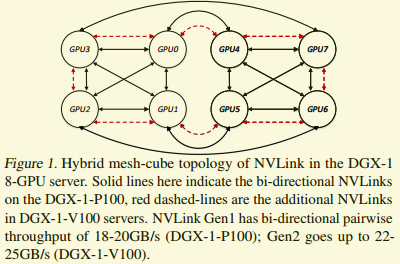
\includegraphics[width=.9\linewidth]{Blink.org_imgs/20201111_092407_ah2YN2.png}
\end{center}
\item 在多租户集群中,对 gpu 之间的互连拓扑是不敏感的。许多 job 被分配到同一个机器上。必须能够利用碎片化时间来避免排队延迟。
\begin{center}
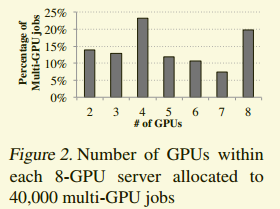
\includegraphics[width=.9\linewidth]{Blink.org_imgs/20201111_093715_mKtQTR.png}
\end{center}
尽管 jobs 大多以2的幂次请求 gpu ,大多数机器还是分配了3,5,6,7个 gpu 。
\end{enumerate}

\textbf{Contributions}:
\begin{itemize}
\item 提出 Blink,以达到接近最佳的链路利用率。
\item 动态生成给定拓扑的最佳通信原语
\item probes the set of links available for a given job at runtime and builds a topology with appropriate link capacities.
\item \ldots{}
\item 提供 NCCL-compatible API, 无缝衔接深度学习框架。
\end{itemize}
\section{MOTIVATION}
\label{sec:org56b6d50}
\subsection{The case for packing trees}
\label{sec:org4b49f4c}
我们的动力来自通信的开销
\subsection{Micro Benchmarks}
\label{sec:org2f0ad64}
\begin{itemize}
\item Depth Test
\begin{itemize}
\item A simple chain topology
\begin{center}
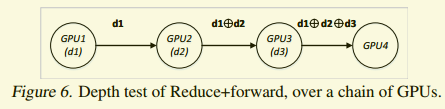
\includegraphics[width=.9\linewidth]{Blink.org_imgs/20201111_192652_Ssn2iX.png}
\end{center}

\begin{center}
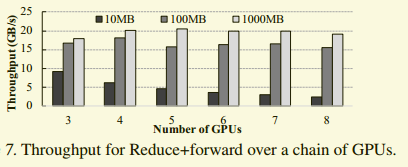
\includegraphics[width=.9\linewidth]{Blink.org_imgs/20201111_192714_5JMvwz.png}
\end{center}
数据集越小,吞吐量下降;chain length 越长(GPU越多),吞吐量从21降到19
\end{itemize}

\item Multi-transfer Test
Two topologies: a multi-input, multi-output (MIMO) as Fig. 8(a) and a multi-chain aggregation (MCA) as Fig. 8(b).
\begin{center}
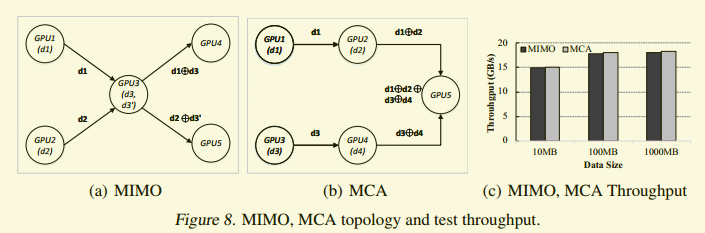
\includegraphics[width=.9\linewidth]{Blink.org_imgs/20201111_193156_SWDr8u.png}
\end{center}
\end{itemize}
\subsection{Blink Approach}
\label{sec:org6f87fa1}
\begin{center}
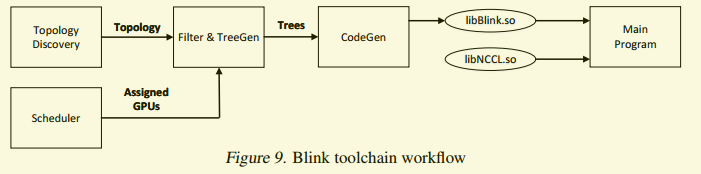
\includegraphics[width=.9\linewidth]{Blink.org_imgs/20201111_200312_t4CsGg.png}
\end{center}
工作流程:
\begin{itemize}
\item 在运行时,一旦深度学习任务被调度并分配了一组gpu, Blink就能够探测机器的拓扑,并通过所分配的 gpu 推断互连拓扑。
\item TreeGen,这一步输出一组生成树和对应于应该通过它们发送多少数据的权重
\item CodeGen parses the spanning trees and generates CUDA code.
\item 设置 LD\textsubscript{PRELOAD} flag,动态加载 Blink 的实现。
\end{itemize}
\section{DESIGN}
\label{sec:org6c39e34}
\subsection{Packing Spanning Trees}
\label{sec:org7c9214f}
GPU, links --> 图论 --> 寻找最大权重的spanning tree
\begin{center}
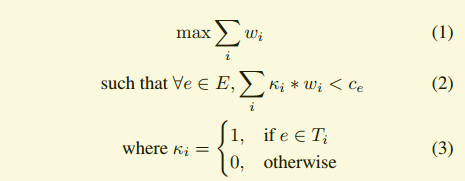
\includegraphics[width=.9\linewidth]{Blink.org_imgs/20201111_201051_Bhhwwu.png}
\end{center}
直接寻找事件复杂度较大,下面介绍优化方法。
\subsection{Approximate Packing}
\label{sec:org61ae8a5}
multiplicative weight update(MWU):
\begin{itemize}
\item 初始化权重和capacity
\item 循环:
\begin{itemize}
\item 寻找最小权重的spanning tree
\item 降低该tree 的权重,更新图的权重
\end{itemize}
\end{itemize}
\subsubsection{Minimizing Number of Trees}
\label{sec:org300e847}
将权重限制为0 or 1 --> 整数线性规划 integer linear program(ILP)
\subsection{Handling many-to-many operations}
\label{sec:org3db7eee}
前面的讨论关注于 one-to-many, 为了解决many-to-many, 我们发现所有机器是双向的,所以图变成了无向图。
\subsection{DGX-2 and Multi-server settings}
\label{sec:org7315e3c}
\section{IMPLEMENTATION}
\label{sec:org773bb70}
\subsection{CodeGen Implementation}
\label{sec:orgd276d13}
简化问题,只讨论两种collective communication: Broadcast and AllReduce
\subsection{CodeGen Optimizations}
\label{sec:org919ae65}
两个问题
\subsubsection{Automatic chunk size selection}
\label{sec:org5a3556a}
块的大小影响整体的效率。
\begin{center}
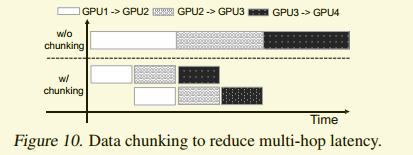
\includegraphics[width=.9\linewidth]{Blink.org_imgs/20201111_202947_MalqKw.png}
\end{center}
使块小点,能够提高系统效率。因此我们需要设计如何自动选择块的大小。

multiplicative increase, additive decrease (MIAD): 初始化块大小很小,当吞吐量提高,以乘法增加块大小,直到达到一个平稳状态。

\begin{center}
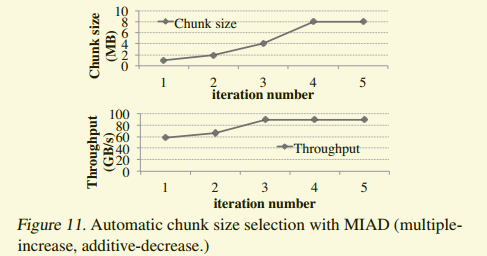
\includegraphics[width=.9\linewidth]{Blink.org_imgs/20201111_203214_5JlRDc.png}
\end{center}
\subsubsection{Link Sharing}
\label{sec:orga80989d}
问题: CUDA functions do not provide any direct control on how links are shared

解决: reusing CUDA streams when the same link is used in multiple trees at roughly the same position
\begin{center}
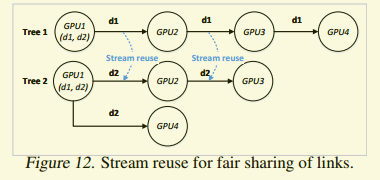
\includegraphics[width=.9\linewidth]{Blink.org_imgs/20201111_203632_FViQuS.png}
\end{center}
\section{EVALUATION}
\label{sec:orgcb2165a}
\subsection{Tree Packing Benefits}
\label{sec:orgaaf5d5e}
\subsection{Broadcast, AllReduce Micro-benchmarks}
\label{sec:org6c5bb2e}
\subsection{End-to-end Training}
\label{sec:org4c01f65}
\section{RELATED WORK}
\label{sec:org83ab016}
\begin{itemize}
\item Topology-fixed Schemes: MPI, Horovod, All-Reduce, Gloo
\item Topology-aware Protocols
\end{itemize}
\section{CONCLUSION}
\label{sec:org27fa493}
Blink是一个用于加速分布式ML的快速通用的集体通信库。为了处理现代GPU硬件中普遍存在的拓扑异构,Blink动态地包生成树以最大化链路利用率。与最先进的基于环的协议(如NCCL2)相比,Blink实现了高达8倍的模型同步,并将端到端训练时间减少了40\%。
\end{document}
